% !TEX root = STP_journal.tex
\subsection{Numerical Simulations \label{sec:basic_results}}
We now illustrate the basic STP algorithm using a four-vehicle example. In this example, we will use the following dynamics for each vehicle:

\begin{equation} \label{eqn:NumSimpleDyn}
\begin{aligned}
\dot{\pos}_{x,i} &= v_i \cos\theta_i \\
\dot{\pos}_{y,i} &= v_i \sin\theta_i \qquad \qquad |\omega_i| \le \bar\omega \\
\dot \theta_i &= \omega_i \\
\end{aligned}
\end{equation}

\noindent where $\state_i = (\pos_{x,i}, \pos_{y,i}, \theta_i)$ is the state of vehicle $\veh_i$, $\pos_i = (\pos_{x,i}, \pos_{y,i})$ is the position, $\theta_i$ is the heading, $v_i$ is the speed, and $\omega_i$ is the turn rate. In this example, we assume that the vehicles have constant speed $v_i = 1 ~ \forall i$, and that the control of each vehicle $\veh_i$ is given by $\ctrl_i = \omega_i$ with $|\omega_i| \le \bar\omega = 1 ~ \forall i$. We have chosen these dynamics for clarity of illustration; STP can handle more general systems of the form in which the vehicles have different control bounds and dynamics. 

For this example, the target sets $\targetset_i$ of the vehicles are circles of radius $r$ in the position space; each vehicle is trying to reach some desired set of positions. In terms of the state space $\state_i$, the target sets are defined as $\targetset_i = \{\state_i: \|\pos_i - c_i\|_2 \le r\}$, where $c_i$ are centers of the target circles. For the simulation of the basic STP algorithm, we used $r = 0.1$. The vehicles have target centers $c_i$, initial conditions $\state_i^0$, and scheduled times of arrivals $\sta_i$ as follows:

\begin{equation} \label{eqn:NumIC}
\begin{aligned}
c_1 = (0.7, 0.2), \quad& \state_1^0 = (-0.5, 0, 0), \quad & \sta_1 = 0 \\
c_2 = (-0.7, 0.2), \quad& \state_2^0 = (0.5, 0, \pi), \quad & \sta_2 = 0.2 \\
c_3 = (0.7, -0.7), \quad& \state_3^0 = \left(-0.6, 0.6, 7\pi/4\right), \quad & \sta_3 = 0.4\\
c_4 = (-0.7, -0.7), \quad & \state_4^0 = \left(0.6, 0.6, 5\pi/4\right), \quad & \sta_4 = 0.6
\end{aligned}
\end{equation}

The setup for this example is shown in Fig. \ref{fig:dubins_ic}, which also shows the static obstacles as the black rectangles around the center of the domain. The joint state space of this four-vehicle system is twelve-dimensional (12D), making the joint trajectory planning and collision avoidance problem intractable for direct analysis using HJ reachability. Therefore, we apply the STP algorithm described in Algorithm \ref{alg:basic} and repeatedly solve the double-obstacle HJ VI in \eqref{eq:HJIVI_BRS} to obtain the optimal control for each vehicle to reach its target while avoiding higher-priority vehicles. In addition, due to the flexibility of the HJ VI with respect to time-varying systems, the different scheduled times of arrival $\sta_i$ can be trivially incorporated. 

Fig. \ref{fig:dubins_reach_all}, \ref{fig:dubins_reach_3}, and \ref{fig:dubins_result} show the simulation results. Since the state space of each vehicle is 3D, each of the BRSs $\brs_i^\text{basic}(t, \sta_i)$ is also 3D. To visualize the results, we slice the BRSs at the initial heading angles $\theta_i^0$. Fig. \ref{fig:dubins_reach_all} shows the 2D BRS slices for each vehicle at its latest departure times $\ldt_1=-1.12, \ldt_2=-0.94,\ldt_3=-1.48,\ldt_4=-1.44$ \textit{determined from our method}. The obstacles in the domain $\soset_i$ and the obstacles induced by higher-priority vehicles $\ioset_i^j(t)$ inhibit the evolution of the BRSs, carving out thin ``channels" that separate the BRSs into different ``islands". One can see how these ``channels'' and ``islands'' form by examining the time evolution of the BRS, shown in Fig. \ref{fig:dubins_reach_3} for vehicle $\veh_3$. 

Finally, Fig. \ref{fig:dubins_result} shows the resulting trajectories of the four vehicles. Most interestingly, the subplot labeled $t=-0.55$ shows all four vehicles in close proximity without collision: each vehicle is outside of the danger zone of all other vehicles (although the danger zones may overlap). This close proximity is an indication of the optimality of the basic STP algorithm given the assigned priority ordering. Since no disturbances are present, getting as close to other vehicles' danger zones as possible without entering the danger zones intuitively results in short transit times.

The actual arrival times of vehicles $\veh_i,i=1,2,3,4$ are $0, 0.19, 0.34, 0.31$, respectively. It is interesting to note that for some vehicles, the actual arrival times are earlier than the scheduled times of arrivals $\sta_i$. This is because in order to arrive at the target by $\sta_i$, these vehicles must depart early enough to avoid major delays resulting from the induced obstacles of other vehicles; these delays would have led to a late arrival if vehicle $\veh_i$ departed after $\ldt_i$.

\begin{figure}
	\centering
	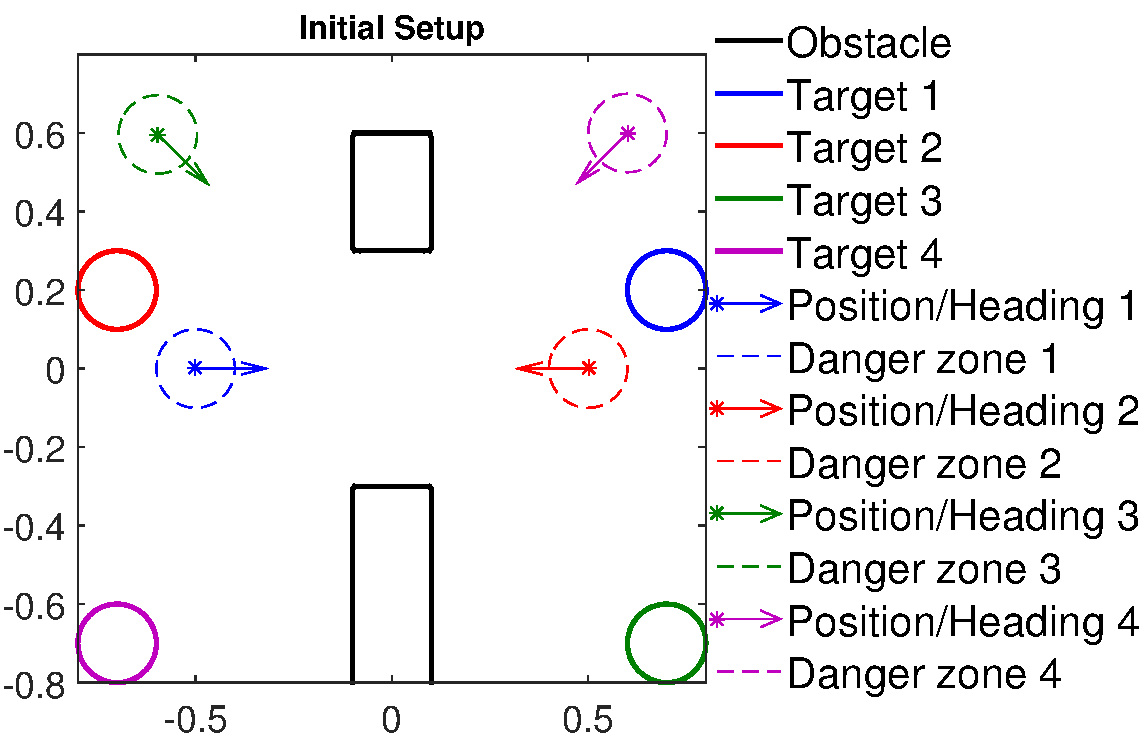
\includegraphics[width=0.6\columnwidth]{fig/dubins_ic}
	\caption{Initial configuration of the four-vehicle example.}
	\label{fig:dubins_ic}
\end{figure}

\begin{figure}
	\centering
	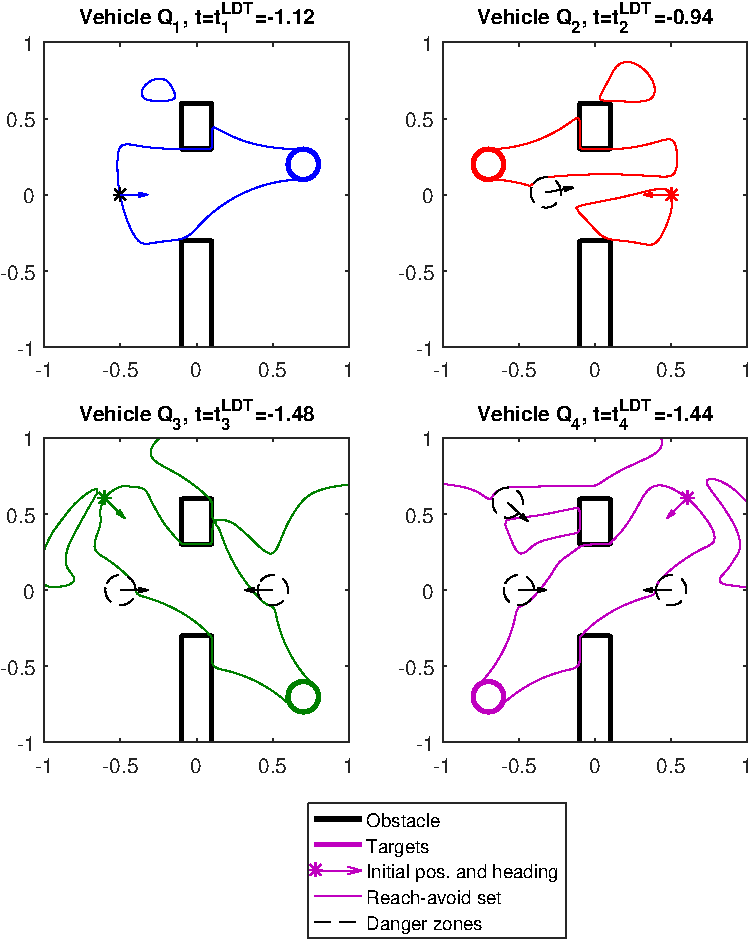
\includegraphics[width=0.8\columnwidth]{fig/dubins_reach_all}
	\caption{BRSs at $t=\ldt_i$ for vehicles $1,2,3,4$, sliced at initial headings $\theta_i^0$. Black arrows indicate direction of obstacle motion. Due to the turn rate constraint, the presence of static obstacles $\soset_i$ and time-varying obstacles induced by higher-priority vehicles $\ioset_i^j(t)$ carve ``channels" in the BRS, dividing it up into multiple ``islands".}
	\label{fig:dubins_reach_all}
\end{figure}

\begin{figure}
	\centering
	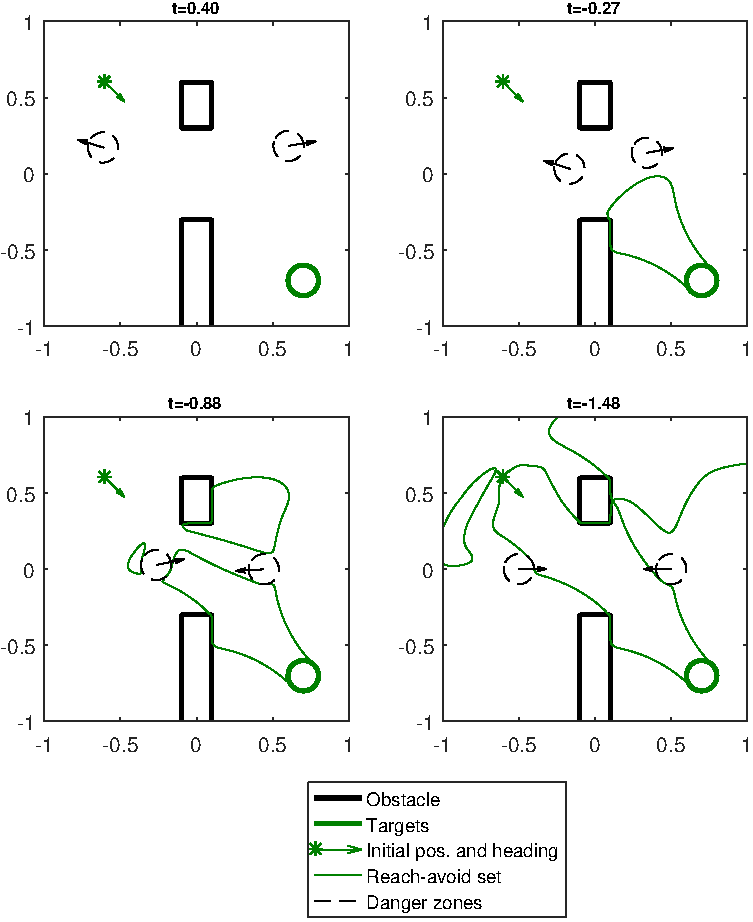
\includegraphics[width=0.8\columnwidth]{fig/dubins_reach_3}
	\caption{Time evolution of the BRS for vehicle $\veh_3$, sliced at its initial heading $\theta_3^0=\frac{7\pi}{4}$. Black arrows indicate direction of obstacle motion. Top row: the BRS grows unobstructed by obstacles (time-varying and static). Bottom row: the static obstacles $\soset_i$ and the induced obstacles $\ioset_3^1,\ioset_3^2$, carve out ``channels" in the BRS.}
	\label{fig:dubins_reach_3}
\end{figure}

\begin{figure}
	\centering
	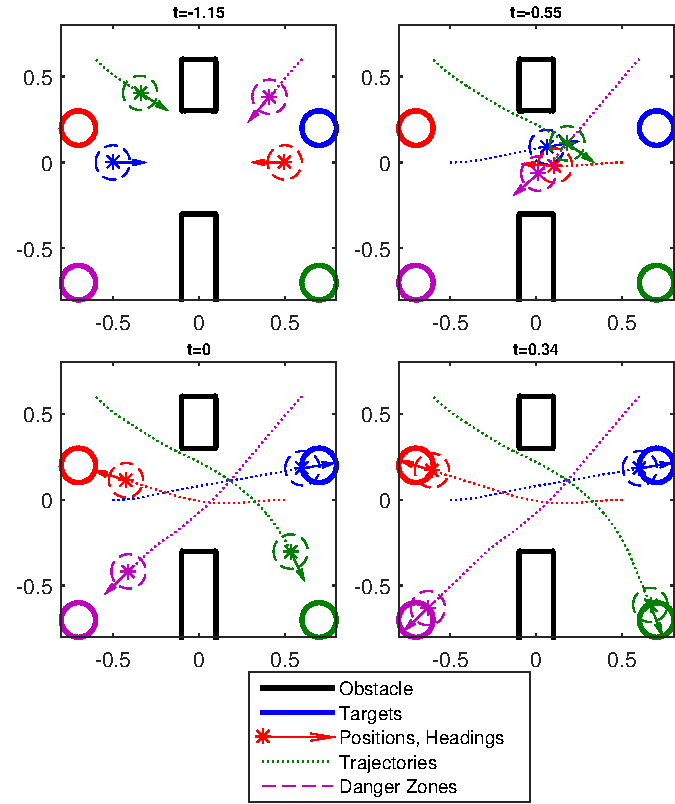
\includegraphics[width=0.8\columnwidth]{fig/dubins_result}
	\caption{The planned trajectories of the four vehicles. Top left: only vehicles $\veh_3$ (green) and $\veh_4$ (purple) have started moving, showing $\ldt_i$ is not common across the vehicles. Top right: all vehicles have come within very close proximity, but none is in the danger zone of another. Bottom left: vehicle $\veh_1$ (blue) arrives at $\targetset_1$ at $t=0$. Bottom right: all vehicles have reached their destination, some ahead of $\sta_i$.}
	\label{fig:dubins_result}
\end{figure}

\MCnote{Computations were done on a desktop computer with a Core i7 5820K processor and two GeForce GTX Titan X graphics processing units. The average computation time per vehicle is approximately 1 second using CUDA and GPU parallelization. Note that for the simulations in this and subsequent sections, almost all of the computation is done offline. Only a look-up table query to obtain the gradient of the value function corresponding to a BRS, and evaluation of the optimal control in, for example \eqref{eq:basicOptCtrl}, is needed online. For control affine systems, controller synthesis amounts to  evaluation of an analytic expression.}